%Introducción a la modulación.

\subsection*{Definiciones de Modulación}
%
\begin{description}
\item[Real Academia] ``Variar con fines armónicos las cualidades del sonido en el habla o en el canto."
\item[Uso clásico en telecomunicaciones] Variar las propiedades (amplitud, frecuencia, fase) de una sinusoide ``portadora" a efectos de transmitir una señal.
\item[Uso moderno, generalizado] Representar información en términos de formas de ondas apropiadas a su transmisión por un canal. Incluye modulación digital.
\end{description}


La operación inversa es la demodulación o detección.

\begin{ejemplo}
Amplitud modulada
\[x_c(t)=\underbrace{A_c\left(1+\mu x(t)\right)}_{\text{\begin{minipage}{2.5cm} $A(t)$  amplitud, depende del mensaje. \end{minipage}}}\cos(2\pi f_c t).\]

\begin{figure}[htb]
\centering
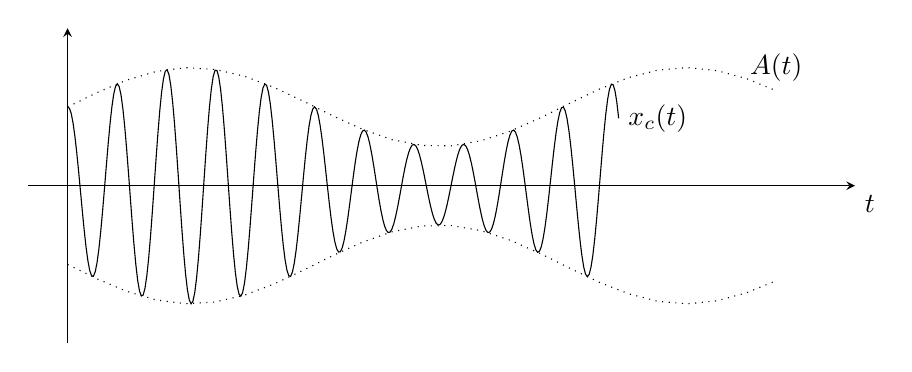
\begin{tikzpicture}
 \draw [-stealth] (0,-2) -- (0,2);
 \draw [-stealth] (-0.5,0) -- (10,0) node [anchor=north west] {$t$};

\draw [domain=0:9, dotted] plot (\x,{1+0.5*sin(\x r)}) node
[anchor=south] {$A(t)$}; \draw [domain=0:9, dotted] plot
(\x,{-1-0.5*sin(\x r)}); \draw [domain=0:7,samples=300] plot
(\x,{(1+0.5*sin(\x r))*cos(10*\x r)}) node [anchor=west]
{$x_c(t)$};
\end{tikzpicture}
\end{figure}

    \begin{itemize}
        \item $x(t)$ varía lentamente, por ejemplo una señal de voz de hasta unos pocos $\unit{\kHz}$.
        \item $f_c \approx 1\,\unit{\MHz}$, mucho más rápido.
    \end{itemize}
\end{ejemplo}

\subsection*{Razones para modular}
\begin{enumerate}
    \item El canal tiene buena propagación en frecuencias cercanas a $f_c$, pero no en la ``banda base'' de $x(t)$.
    \item \label{raz2} Permite el multiplexado en frecuencia, compartir el canal.
\end{enumerate}

Para ver lo primero, usamos la Transformada de Fourier,
$x(t)\xrightarrow{\mathcal{F}}\hat{X}(f)$.
\begin{figure}[htb]
    \centering
    \begin{tikzpicture}[xscale=2.5,yscale=1.5]
        \draw [-stealth] (-1.5,0) -- (1.5,0) node [anchor=north] {\footnotesize $f$};
        \draw [-stealth] (0,-0.3) -- (0,2) node [anchor=west] {\footnotesize $\hat{X}(f)$};
        \specfull{0}
        \path (1,0) node [anchor=north] {\footnotesize $\sim 1\,\unit{\kHz}$};
    \end{tikzpicture}
\end{figure}
\FloatBarrier

Usando la propiedad de modulación de la Transformada de Fourier,
tenemos:
\[\hat{X}_c(f)=\frac{A_c}{2}\left[\delta(f+f_c)+\delta(f-f_c)+\mu\hat{X}(f+f_c)+\mu\hat{X}(f-f_c)\right].\]

\begin{figure}[htb]
    \centering
    \begin{tikzpicture}[xscale=1.5]
        \draw [-stealth] (-4,0) -- (4,0) node [anchor=north] {\footnotesize $f$};
        \draw [-stealth] (0,-0.3) -- (0,3) node [anchor=west] {\footnotesize $\hat{X}_c(f)$};
        \specfull{-2.5}
        \specfull{2.5}
        \draw [-stealth,very thick] (-2.5,0) node [anchor=north] {\footnotesize $-f_c$} -- (-2.5,2);
        \draw [-stealth,very thick] (2.5,0) node [anchor=north] {\footnotesize  $f_c\sim 1\,\unit{\MHz}$} -- (2.5,2) node [anchor=south west] {$\left(\dfrac{A_c}{2}\right)$};
    \end{tikzpicture}
\end{figure}
\FloatBarrier

Un canal de radio tiene buena propagación en $f\sim 1\,\unit{\MHz}$, no
así en $f\sim 1\,\unit{\kHz}$
 (esto requeriría antenas de $\sim 100\,Km$). Por tanto, la modulación adapta la señal al canal.

El {\em multiplexado en frecuencia} consiste en que dos ondas
comparten el mismo canal con diferentes $f_c$. Por ejemplo, sean
dos antenas de radio que transmiten a frecuencias
$f_{c_1}=770\,\unit{\kHz}$ y $f_{c_2}=810\,\unit{\kHz}$. Las señales transmitidas
respectivamente por cada antena son
\begin{align*}
x_{c1}(t)&=A_{c1}\left(1+\mu_1x_1(t)\right)\cos(2\pi f_{c_1}t),\\
x_{c2}(t)&=A_{c2}\left(1+\mu_2x_2(t)\right)\cos(2\pi f_{c_2}t).
\end{align*}
Si cada señal se encuentra sometida a una atenuación $K_1$ y $K_2$
antes de llegar al receptor, la señal recibida por éste es
\[x_R(t)=x_{R_1}(t)+x_{R_2}(t)=K_1x_{c1}(t)+K_2x_{c2}(t).\]
Graficamos su espectro de Fourier.

\begin{figure}[htb]
    \centering
    \begin{tikzpicture}[scale=1.1]
        \draw [-stealth] (-6,0) -- (6,0) node [anchor=north] {\footnotesize $f$};
        \draw [-stealth] (0,-8.5) -- (0,2) node [anchor=west] {\footnotesize $\hat{X}_1(f)$};
        \specfull{0}
        \path (-0.95,0) node[anchor=north] {\footnotesize $-B$} -- (0.95,0) node[anchor=north]{\footnotesize $B$};
        \begin{scope}[shift={(0,-2)}]
            \draw [-stealth] (-6,0) -- (6,0) node [anchor=north]{\footnotesize $f$};
            \specfull{-2.5}
            \specfull{2.5}
            \draw [-stealth,thick] (-2.5,0) node [anchor=north] {\footnotesize $-f_{c_1}$} -- (-2.5,1.5);
            \draw [-stealth,thick] (2.5,0) node [anchor=north] {\footnotesize $f_{c_1}$} -- (2.5,1.5);
            \path (0,1) node [anchor=west] {\footnotesize $\hat{X}_{R_1}(f)$};
        \end{scope}
        \begin{scope}[shift={(0,-4)}]
            \draw [-stealth] (-6,0) -- (6,0) node [anchor=north]{\footnotesize $f$};
            \draw (-0.9,0) -- (0,0.9) -- (0.9,0);
            \path (0,1) node [anchor=west] {\footnotesize $\hat{X}_2(f)$};
        \end{scope}
        \begin{scope}[shift={(0,-6)}]
            \draw [-stealth] (-6,0) -- (6,0) node [anchor=north]{\footnotesize $f$};
            \draw (-5.4,0) -- (-4.5,0.9) -- (-3.6,0);
            \draw (3.6,0) -- (4.5,0.9) -- (5.4,0);
            \path (0,1) node [anchor=west] {\footnotesize $\hat{X}_{R_2}(f)$};
            \draw [-stealth,thick] (-4.5,0) node [anchor=north] {\footnotesize $-f_{c_2}$} -- (-4.5,1.5);
            \draw [-stealth,thick] (4.5,0) node [anchor=north] {\footnotesize $f_{c_2}$} -- (4.5,1.5);
        \end{scope}
        \begin{scope}[shift={(0,-8)}]
            \draw [-stealth] (-6,0) -- (6,0) node [anchor=north]{\footnotesize $f$};

            \draw (-5.4,0) -- (-4.5,0.9) -- (-3.6,0);
            \draw (3.6,0) -- (4.5,0.9) -- (5.4,0);
            \draw [-stealth,thick] (-4.5,0) node [anchor=north] {\footnotesize $-f_{c_2}$} -- (-4.5,1.5);
            \draw [-stealth,thick] (4.5,0) node [anchor=north] {\footnotesize $f_{c_2}$} -- (4.5,1.5);

            \specfull{-2.5}
            \specfull{2.5}
            \draw [-stealth,thick] (-2.5,0) node [anchor=north] {\footnotesize $-f_{c_1}$} -- (-2.5,1.5);
            \draw [-stealth,thick] (2.5,0) node [anchor=north] {$\footnotesize f_{c_1}$} -- (2.5,1.5);

            \path (0,1) node [anchor=west] {\footnotesize $\hat{X}_R(f)$};
        \end{scope}

        \draw [dotted] (-5.4,-6) -- (-5.4,-8);
        \draw [dotted] (-3.6,-6) -- (-3.6,-8);

        \draw [dotted] (5.4,-6) -- (5.4,-8);
        \draw [dotted] (3.6,-6) -- (3.6,-8);

        \draw [dotted] (-3.45,-2) -- (-3.45,-8);
        \draw [dotted] (-1.55,-2) -- (-1.55,-8);

        \draw [dotted] (3.45,-2) -- (3.45,-8);
        \draw [dotted] (1.55,-2) -- (1.55,-8);
    \end{tikzpicture}
\end{figure}
\FloatBarrier

Si los canales no se solapan en frecuencia, puedo seleccionar uno
de ellos mediante un filtrado selectivo, entonces escucho una sola
radio. 

Faltaría ver como recuperar el mensaje $x(t)$ de la onda modulada, para esto hacemos uso de una demodulación o detección.

En el caso de AM, lo más sencillo es un ``detector de envolvente''
que extrae la amplitud $A(t)=\left(1+\mu x(t)\right)$ de la onda
modulada. $A(t)$ es proporcional al mensaje, a menos de un
término de continua que puede eliminarse.

En este curso se estudiará la modulación \emph{digital},
donde el mensaje $x(t)$ es una sucesión de símbolos. Se busca como
mejor representarlos a efectos de su transmisión por un canal.
Aquí también analizaremos la eficiencia espectral y el impacto del
ruido.